\begin{frame}{Introduction}
En physique, les modèles prévoient les valeurs de quantités mesurables, appelées \textbf{observables}. Ce sont des fonctions
\[f:\Omega \rightarrow \R\]
où $\Omega$ est l'espace de configuration du système. Ces observables commutent en physique classique.\\
\vspace{0.3 cm} 
Pour donner un modèle de l'atome d'hydrogène en accord avec l'expérience, Heisenberg propose en 1925 de remplacer les observables classiques par des "q-nombres", qui ne commutent pas.
\[pq -qp = i\hbar 1\]
\end{frame}

\begin{frame}{Introduction}
Les "nombres" utilisés en physique quantique forment une algèbre d'opérateurs. Ces algèbres sont encodées d'un point de vue abstrait par la notion de $C^*$-algèbre. 
\vspace{0.3 cm}
\begin{definitionfr}
Une $C^*$-algèbre est une $\C$-algèbre $A$ munie d'un antihomomorphisme involutif $*$ et d'une norme multiplicative $||.||$ telle que :
\begin{itemize}
\item[$\bullet$] $(A,||.||)$ est une algèbre de Banach,
\item[$\bullet$] $||a^*a||^2 = ||a||^2$ pour tout $a\in A$.
\end{itemize}
\end{definitionfr}

\begin{itemize}
\item[$\bullet$] l'algèbre des opérateurs bornés sur un espace de Hilbert $\mathcal L(H)$, 
\item[$\bullet$] l'algèbre des fonctions continues sur un espace localement compact $C_0(X)$.
\end{itemize}

\end{frame}

\begin{frame}{Introduction}
Il s'avère que toute $C^*$-algèbre commutative est équivalente à un espace localement compact.
\begin{thmfr}[Dualité de Gelfand]
Soit $A$ une $C^*$-algèbre commutative. Alors il existe un espace localement compact $X$ et un $*$-isomorphisme 
\[A\cong C_0(X).\]
\end{thmfr}

Alain Connes développe à partir des années 80 la géométrie non-commutative basée sur le principe suivant
\begin{block}{Géométrie Non-Commutative}
Une $C^*$-algèbre représente un "espace non-commutatif". 
\end{block}

\end{frame}

\begin{frame}{Introduction}
L'idée des physiciens (remplacer l'algèbre des coordonnées par une algèbre d'opérateurs) peut être utilisée pour étudier des espaces pathologiques.
\vspace{0.3 cm}
\begin{block}{Philosophie}
Associer à une situation géométrique une $C^*$-algèbre.
\end{block}
\vspace{0.3 cm}
Quels espaces pathologiques ? Principalement, des espaces d'orbites, associés à :
\begin{itemize}
\item[$\bullet$] des actions de groupes,
\item[$\bullet$] des feuilletages,
\item[$\bullet$] des sytèmes dynamiques.
\end{itemize} 
\end{frame}

\begin{frame}{Introduction}
\textbf{Exemple :} Le groupe $\Z$ agit sur le cercle $\mathbb S^1$ par rotation d'angle $2\pi\theta$.
\vspace{0.3 cm}
\[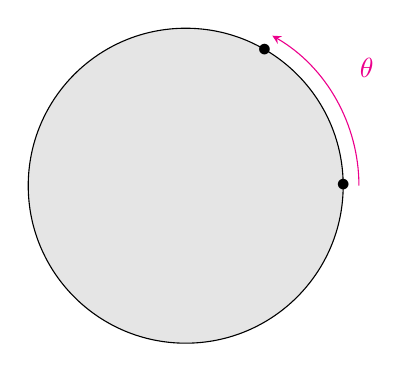
\begin{tikzpicture}
\draw[fill = gray!20] (0,0) circle (2) ;
\draw [>=stealth, ->, magenta] (2.2,0)  arc (0:60:2.2); %--(1 , 1.72);
\draw[magenta]  (2.3,1.5) node {$\theta$};
\draw  (2,0) node {$\bullet$};
\draw  (1,1.72) node {$\bullet$};
\end{tikzpicture}\]
\end{frame}

\begin{frame}{Introduction}
Deux cas :
\vspace{0.3 cm}
\begin{itemize}
\item[$\bullet$] $\theta\in \mathbb Q$ : les orbites sont périodiques, et le quotient est 
\[\mathbb S^1 / \Z \cong \mathbb S^1,\] 
\item[$\bullet$] $\theta \notin \mathbb Q$ : toute orbite est dense, et  $\mathbb S^1 / \Z$ est un espace hautement pathologique. Rien ne le distingue d'un point.
 \[C_0(\mathbb S^1 / \Z) \cong \C.\]
\end{itemize}
\vspace{0.3 cm}
Une solution : construire un groupoïde qui encode la situation géométrique. On sait associer des $C^*$-algèbres aux groupoïdes.\\
\end{frame}

\begin{frame}{Introduction}

\vspace{0.3 cm}
\begin{definitionfr}[Groupoïde]
Un groupoïde est la donnée de deux espaces topologiques, l'espace des flèches $G$ et celui des unités $G^{(0)}$, ainsi que de :
\begin{itemize}
\item[$\bullet$] un plongement topologique $e: G^{(0)} \rightarrow G; x\mapsto e_x$, 
\item[$\bullet$] des applications continues surjectives source et but $s,r : G\rightrightarrows G^{(0)}$ telles que $r\circ e =s\circ e = id_{G^{(0)}}$,
\item[$\bullet$] une multiplication continue \[G^{(2)}=G\times_{s,r} G\rightarrow G; (g,g') \mapsto gg'\] 
telle que $g(g'g'') = (gg')g''$ et $ge_{s(g)} = e_{r(g)}g= g$,
\item[$\bullet$] une involution continue $G\rightarrow G ; g\mapsto g^{-1}$ telle que $gg^{-1} = e_{r(g)}$, $g^{-1}g = e_{s(g)}$ et $s(g^{-1})=r(g)$.	
\end{itemize}
\end{definitionfr}
\end{frame}

\begin{frame}{Introduction}
\[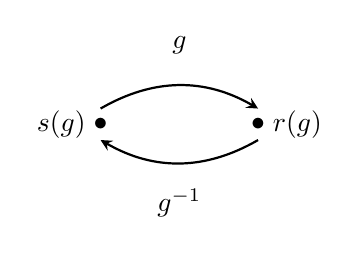
\begin{tikzpicture}
\draw  (0,1) node {$g$};
\draw  (0,-1) node {$g^{-1}$};
\draw [>=stealth, ->, thick] (-1,0.2) to[bend left] (1,0.2);
\draw [>=stealth, ->,thick] (1,-0.2) to[bend left] (-1,-0.2);
\draw  (-1,0) node {$\bullet$};
\draw  (-1.5,0) node {$s(g)$};
\draw  (1,0) node {$\bullet$};
\draw  (1.5,0) node {$r(g)$};
\end{tikzpicture}\]
\end{frame}

\begin{frame}{Introduction}
Des exemples de groupoïdes :
\vspace{0.3 cm}
\begin{itemize}
\item[$\bullet$] un espace topologique $X\rightrightarrows X$,
\item[$\bullet$] un groupe topologique $G\rightrightarrows *$,
\item[$\bullet$] le groupoïde des paires $X\times X\rightrightarrows X$,
\[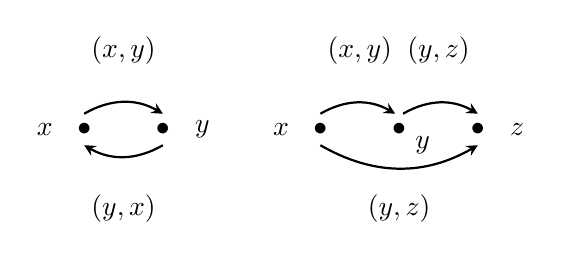
\begin{tikzpicture}
\draw  (-2,1) node {$(x,y)$};
\draw  (-2,-1) node {$(y,x)$};

\draw  (1,1) node {$(x,y)$};
\draw  (2,1) node {$(y,z)$};
\draw  (1.5,-1) node {$(y,z)$};

\draw [>=stealth, ->, thick] (-2.5,0.2) to[bend left] (-1.5,0.2);
\draw [>=stealth, ->,thick] (-1.5,-0.2) to[bend left] (-2.5,-0.2);

\draw [>=stealth, ->, thick] (0.5,0.2) to[bend left] (1.45,0.2);
\draw [>=stealth, ->, thick] (1.55,0.2) to[bend left] (2.5,0.2);
\draw [>=stealth, ->, thick] (0.5,-0.2) to[bend right] (2.5,-0.2);


\draw  (-2.5,0) node {$\bullet$};
\draw  (-1.5,0) node {$\bullet$};
\draw  (0.5,0) node {$\bullet$};
\draw  (1.5,0) node {$\bullet$};
\draw  (2.5,0) node {$\bullet$};

\draw  (-3,0) node {$x$};
\draw  (-1,0) node {$y$};
\draw  (0,0) node {$x$};
\draw  (1.8,-0.2) node {$y$};
\draw  (3,0) node {$z$};
\end{tikzpicture}\]
\item[$\bullet$] le dernier exemple se généralise aux relations d'équivalence : $R\subseteq X\times X$.
\end{itemize}
\end{frame}

\begin{frame}{Introduction}
$\bullet$ Soit $\Gamma$ un groupe dénombrable discret agissant sur $X$ par homéomorphismes. Le groupoïde produit croisé noté $X\rtimes \Gamma \rightrightarrows X$.
\[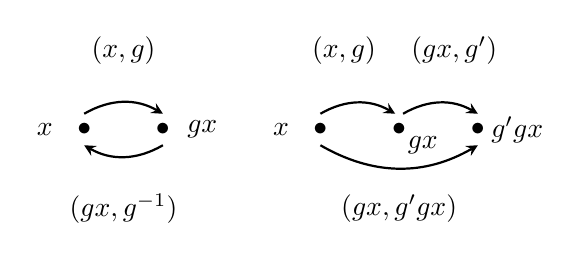
\begin{tikzpicture}
\draw  (-2,1) node {$(x,g)$};
\draw  (-2,-1) node {$(gx,g^{-1})$};

\draw  (0.8,1) node {$(x,g)$};
\draw  (2.2,1) node {$(gx,g')$};
\draw  (1.5,-1) node {$(gx,g'gx)$};

\draw [>=stealth, ->, thick] (-2.5,0.2) to[bend left] (-1.5,0.2);
\draw [>=stealth, ->,thick] (-1.5,-0.2) to[bend left] (-2.5,-0.2);

\draw [>=stealth, ->, thick] (0.5,0.2) to[bend left] (1.45,0.2);
\draw [>=stealth, ->, thick] (1.55,0.2) to[bend left] (2.5,0.2);
\draw [>=stealth, ->, thick] (0.5,-0.2) to[bend right] (2.5,-0.2);


\draw  (-2.5,0) node {$\bullet$};
\draw  (-1.5,0) node {$\bullet$};
\draw  (0.5,0) node {$\bullet$};
\draw  (1.5,0) node {$\bullet$};
\draw  (2.5,0) node {$\bullet$};

\draw  (-3,0) node {$x$};
\draw  (-1,0) node {$gx$};
\draw  (0,0) node {$x$};
\draw  (1.8,-0.2) node {$gx$};
\draw  (3,0) node {$g'gx$};
\end{tikzpicture}\]
\end{frame}

\begin{frame}{Introduction}
Quelques $C^*$-algèbres associées :
\vspace{0.3 cm}
\begin{itemize}
\item[$\bullet$] $C_r^*(X)\cong C_0(X)$,
\vspace{0.3 cm}
\item[$\bullet$] dans le cas d'un groupe, on retrouve la $C^*$-algèbre de groupe,
\vspace{0.3 cm}
\item[$\bullet$] si $X$ est fini, $C^*_r(X\times X) \cong \mathcal L (l^2(X)) \cong \mathfrak M_{|X|}(\C)$,
\vspace{0.3 cm}
\item[$\bullet$] $C^*_r(X\rtimes \Gamma) \cong C_0(X)\rtimes_r \Gamma$.
\end{itemize}
\end{frame}

\begin{frame}{Introduction}
Dans le cas de la topologie classique, un des objets à déterminer est ce qu'on appelle l'homologie et la cohomologie d'un espace.\\
\vspace{0.3 cm}
Dans le cadre de la géométrie non-commutative, on voudra déterminer la $K$-théorie des certaines $C^*$-algèbres, qui est l'analogue des théories homologiques classiques. 
\vspace{0.3 cm}
\begin{block}{Objectif de la thèse}
Déterminer les groupes de $K$-théorie de certaines familles de $C^*$-algèbres.
\end{block}
\end{frame}

\begin{frame}{Introduction}
Pour cela, voici notre stratégie :\\
\vspace{0.3 cm}
\begin{itemize}
\item[$\bullet$] détecter la filtration naturelles des produits croisés de $C^*$-algèbres par des groupoîdes étales et des groupes quantiques discrets,
\vspace{0.3 cm}
\item[$\bullet$] approximer la $K$-théorie par la $K$-théorie contrôlée,
\vspace{0.3 cm}
\item[$\bullet$] dans le cas des $C^*$-algèbres de Roe et des produits croisés de groupoïdes étales, construire des applications d'assemblage,
\vspace{0.3 cm}
\item[$\bullet$] prouver une version contrôlée de la conjecture de Baum-Connes.
\end{itemize}
\end{frame}
